\documentclass[FyPI.tex]{subfiles}

\begin{document}

\chapter{Fractales. Introducción.}
\section{Apuñalar a esos profesores que no dan apuntes}
No existe una definición aceptada de lo que es un objeto fractal, aunque se acepta comúnmente que los fractales deben tener ciertas características.
\begin{enumerate}
\item Poseen \textbf{autosemjanza} o \textbf{autosimilitud}, ya sea general o por zonas.
\item Tienen una \textbf{dimensión fractal}, que será mayor o igual que su dimensión topológica.
\item Son conjuntos, en cierto sentido, \textbf{irregulares}.
\end{enumerate}
\section{Conjunto de Cantor}
Consideremos el intervalo $[0,1]$. Realizamos un proceso iterativo en el que dividimos el conjunto en tres partes iguales y eliminamos la parte de en medio. Aplicamos iterativamente este procedimiento a los suscesivos intervalos que se van generando. 
\begin{figure}[h!]
\centering
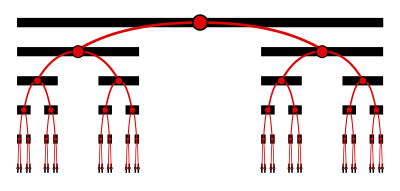
\includegraphics[scale=0.7]{prueba}
\end{figure}
Para codificar estos intervalos, vamos a notar a los intervalos de la siguiente manera. En la primera división llamamos al primer intervalo $I_0$ y al segundo $I_1$, y a su unión $C_1$. A los cuatro siguientes, $I_{00}$, $I_{01}$, $I_{10}$ e $I_{11}$, y a la unión $C_2$. Y así, sucesivamente.

El conjunto de cantor es la intersección de todos los $C_i$ y, al estar encajados, es de hecho el límite de los $C_i$. Notemos que $\forall i \geq 1$ $C_i \subset C_{i-1}$. Denotamos por $C$ el conjunto de Cantor. 
\newpage
Vamos a calcular la longitud de $C$. Notemos que
$$
m(C_i) = \left(\frac{2}{3}\right)^i \qquad \lim_{i\to\infty} m(C_i) = 0
$$
Dado que $C\subset C_i$  y la medida $m(\cdot)$ es monótona y no negativa, se tiene que $m(C)=0$.

Una vez vista su medida, pasamos a ver su cardinalidad. Recordemos que $\forall x \in [0,1]$ 
$$
x = \sum_{n=1}^\infty \frac{a_n}{3^n} \quad a_n\in \{0,1,2\}
$$
Aunque esta representación no es única, pues
$$
\frac{1}{3} = \sum_{n=2}^\infty \frac{2}{3^n}
$$
Lo que sí es cierto con respecto a esta dualidad es que cualquier $x$ que tenga un representación finita también va a tener una representación infinita. Puede probarse que
$$
C=\{0\}\cup\{x\in(0,1] \mid x = \sum_{n=1}^\infty \frac{a_n}{3^n},\text{ suma infinita, }\;a_n = 0,2,\; n \in \mathbb{N}\}
$$
Antes de continuar, tenemos que saber que en la literatura matemática es frecuente encontrar que el conjunto
$$
C=\{0,1\}^\mathbb{N} = \{f:\mathbb{N} \to \{0,1\}\} = \{(\varepsilon_1,\varepsilon_2,\dotsc)\mid \varepsilon_i \in \{0,1\}\}
$$
es denominado conjunto de Cantor. Vamos a definir una aplicación que conecte ambos conjuntos de Cantor:
$$
\phi(\varepsilon_1,\varepsilon_2,\dotsc) = \sum_{n=1}^\infty \frac{2\varepsilon_n}{3^n}
$$
Se puede probar que $\phi$ es una biyección. Además, este nuevo conjunto de cantor tiene una biyección trivial con $\R$, a saber
$$
f:\{0,1\}^\mathbb{N} \to [0,1] \qquad (\varepsilon_1,\varepsilon_2,\dotsc) \to \sum_{n=1}^{\infty} \frac{\varepsilon_n}{2^n}
$$
Por tanto, el conjunto de Cantor tiene cardinalidad infinita no numerable.

Veamos otra forma de reproducir el conjunto de Cantor. Partamos del intervalo $I=\{0,1\}$, aunque podríamos utilzar otro. Definimos las aplicaciones
\begin{align*}
T_0& : [0,1]\to [0,1] & T_1&:[0,1]\to [0,1] \\
x& \to \frac{1}{3}x & x &\to \frac{1}{3}x+\frac{2}{3}
\end{align*}
Naturalmente $T_0(I) = [0,1/3]$ y $T_1(I)=[2/3,1]$. Definimos $T(A)=T_0(A)\cup T_1(A)$. Por tanto
$$
T(C_1) = T_0(C_1)\cup T_1(C_1) = C_2, \qquad T(C_n) = C_{n+1}
$$
\section{Triángulo de Sierpinski}
 Partimos de un triángulo, en principio equilatero aunque no tiene por qué. Dividimos en cuatro triángulos iguales y desechamos el interior. Comenzando por el que corresponde a la base en el lado izquierdo numeramos en sentido contrario a las agujas del reloj $E_0$, $E_1$ y $E_2$ análogamente a como hicimos en el conjunto de Cantor. Repetimos iterativamente el proceso sobre estos triángulos. Podemos considerar los conjuntos $E_{00}$, $E_{01}$, $E_{02}$, $E_{10}$, etc. Así, denotamos
$$
S_1 = E_0 \cup E_1 \cup E_2 \qquad S_2 = \bigcup_{e_1,e_2 \in \{0,1,2\}} E_{e_1 e_2}
$$
y análogamente definimos $S_n$. Naturalmente $S_n \subset S_{n-1}$ para $n\geq 1$. Denominamos Triángulo de Sierpinski a la intersección de todos ellos. Se puede probar que el conjunto es no vacío y de cardinalidad no numerable. Se puede probar que $m(S) = 0$ como subconjunto de $\R^2$ usando que $m(S_n)=\left(\dfrac{3}{4}\right)^n$.
\begin{figure}[h!]
\centering
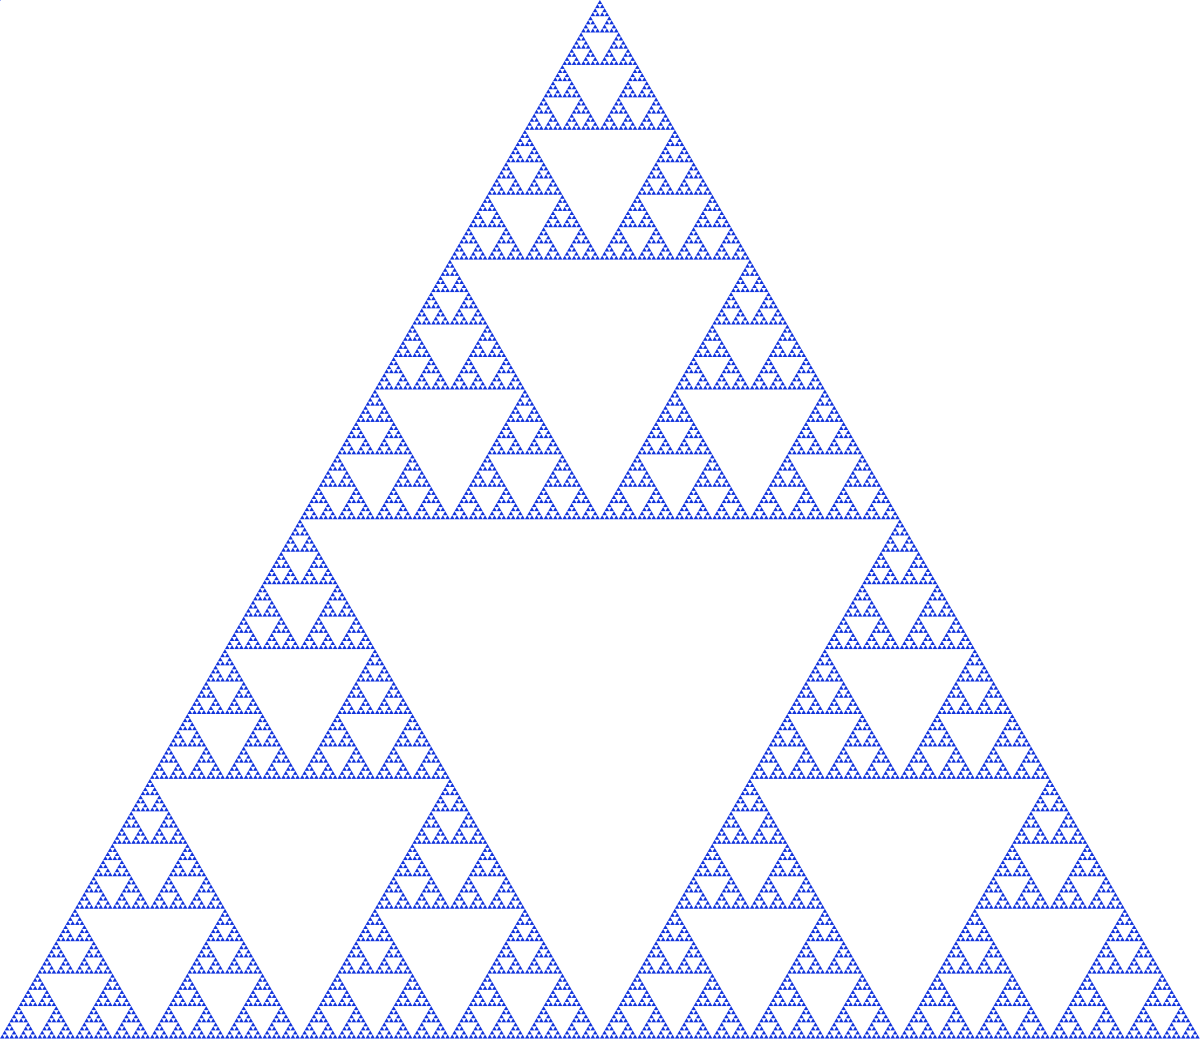
\includegraphics[scale=0.2]{sierpi}
\end{figure}

Otra forma de reproducir este conjunto es considerar $S$ el triángulo equilatero cuya base está en $[0,1]$ y está en el primer cuadrante. 
\begin{align*}
T_0 &: S\to S & T_1&:S\to S & T_2&: S\to S \\
(x,y)& \to \frac{1}{2}(x,y) & (x,y) &\to \frac{1}{2}+ (1/2,0) & (x,y) & \to \frac{1}{2} (x,y)+(1/4,\sqrt{3}/4)
\end{align*}
Si definimos $T(A) = T_0(A)\cup T_1(A)\cup T_2(A)$ entonces $T(S) = S_1$, $T(S_1) = S_2$ y, en general, $T(S_n) = S_{n+1}$.


\chapter{Sistema de funciones iteradas}
\section{Espacio métrico}
\begin{defi}
Sea $X$ un conjunto. Una \textbf{métrica} o \textbf{distancia }en $X$ es una aplicación $d: X\times X \to [0,\infty)$ que verifica
\begin{itemize}
\item Si $x=y$ si y solo si $d(x,y)=0$.
\item La aplicación es simétrica, es decir, $\forall x,y\in X$ $d(x,y)=d(y,x)$.
\item Se verifica la desigualdad triangular, es decir, $\forall x,y,z \in X$ 
$$
d(x,y)\leq d(x,z)+d(z,y)
$$
\end{itemize}
\end{defi}
\begin{defi}
Diremos que $(X,d)$ es un espacio métrico si $X$ es un conjunto y $d$ es una distancia en $X$.
\end{defi}
\begin{nota}
Sea $x\in X$, $\varepsilon >0$. Denotamos
$$
B(x,\varepsilon) = \{y \in X \mid d(x,y)<\varepsilon\}
$$
\begin{defi}
Sea $A\subset X$. Diremos que $A$ es \textbf{abierto} si $\forall x \in A$ $\exists \varepsilon>0$ tal que $B(x,\varepsilon)\subset A$. Diremos que $A$ es \textbf{cerrado} si $A^c$ es abierto.
\end{defi}
\end{nota}
\end{document}
